% =========================================================================
%  Biological Penalty Sharpness Bounds the Value of In-Season Replanning
%  in Multi-Field Hybrid Maize Seed Production
%
%  NOTE ON FORMAT: this file reproduces IEEEtran conference style using the
%  standard article class, so it compiles without IEEEtran.cls installed.
%  Conventions follow the supplied reference paper: full-width roman title,
%  a grid of author blocks, bold abstract and index terms with run-in italic
%  labels, centred small-caps section headings, "TABLE N" plus a small-caps
%  caption set ABOVE each table, and "Fig. N." captions set BELOW figures.
%  To submit, drop the body into the conference's official IEEEtran template.
% =========================================================================
\documentclass[10pt,twocolumn]{article}

\usepackage[letterpaper,top=0.75in,bottom=1.0in,left=0.625in,right=0.625in,
            columnsep=0.25in]{geometry}
\usepackage{times}
\usepackage{amsmath,amssymb}
\usepackage{graphicx}
\usepackage{booktabs}
\usepackage{algorithm}
\usepackage{algorithmic}
\usepackage{xcolor}
\definecolor{ieeelink}{rgb}{0.25,0.42,0.70}
\usepackage[hidelinks]{hyperref}
\Urlmuskip=0mu plus 0.3mu\relax
\def\UrlBreaks{\do\/\do\-\do\.\do\_\do\?\do\=\do\&\do\a\do\b\do\c\do\d\do\e\do\f\do\g\do\h\do\i\do\j\do\k\do\l\do\m\do\n\do\o\do\p\do\q\do\r\do\s\do\t\do\u\do\v\do\w\do\x\do\y\do\z}
\usepackage[labelsep=period]{caption}
\usepackage{titlesec}
\usepackage{balance}
\usepackage{fancyhdr}

\setlength{\parindent}{1em}
\raggedbottom
\setlength{\abovedisplayskip}{4pt}
\setlength{\belowdisplayskip}{4pt}

% ---- section headings: centred, small caps, Roman numerals -------------
\renewcommand{\thesection}{\Roman{section}}
\renewcommand{\thesubsection}{\Alph{subsection}}
\makeatletter\renewcommand{\p@subsection}{\thesection-}\makeatother
\renewcommand{\thesubsubsection}{\arabic{subsubsection}}

\titleformat{\section}[block]
  {\normalfont\normalsize\centering\scshape}{\thesection.}{0.5em}{}
\titlespacing*{\section}{0pt}{10pt plus 2pt minus 2pt}{6pt}

\titleformat{\subsection}[block]
  {\normalfont\normalsize\itshape}{\thesubsection.}{0.6em}{}
\titlespacing*{\subsection}{0pt}{8pt plus 1pt minus 1pt}{4pt}

\titleformat{\subsubsection}[runin]
  {\normalfont\normalsize\itshape}{\thesubsubsection)}{0.5em}{}[:]
\titlespacing*{\subsubsection}{\parindent}{4pt}{0.5em}

% ---- captions: tables above in small caps, figures below ---------------
\captionsetup[table]{position=top,labelsep=newline,justification=centering,
                     font=sc,labelfont=sc,skip=3pt,textformat=simple}
\captionsetup[figure]{position=bottom,font=small,labelfont=normalfont,
                      labelsep=period,skip=5pt,justification=justified}
\renewcommand{\tablename}{Table}
\renewcommand{\thetable}{\Roman{table}}
\renewcommand{\figurename}{Fig.}

% ---- tighter float separation -----------------------------------------
\setlength{\textfloatsep}{7pt plus 2pt minus 2pt}
\setlength{\floatsep}{6pt plus 2pt minus 2pt}
\setlength{\intextsep}{6pt plus 2pt minus 2pt}
\setlength{\dbltextfloatsep}{7pt plus 2pt minus 2pt}
\setlength{\dblfloatsep}{6pt plus 2pt minus 2pt}

% ---- IEEE-style run-in abstract (no centred heading, no extra margins) --
\renewenvironment{abstract}
  {\small\bfseries\noindent\textit{Abstract}---\ignorespaces}
  {\par}

\newcommand{\TSI}{\mathrm{TSI}}
\newcommand{\EVPI}{\mathrm{EVPI}}
\newcommand{\VSS}{\mathrm{VSS}}

% ---- title block -------------------------------------------------------
\title{\vspace{-2.2em}\normalfont\LARGE
Optimised Sowing Scheduling for Multi-Field\\
Hybrid Maize Seed Production under\\
Anthesis-Synchrony Constraints}

% Author block in the IEEE conference template form: one block per author,
% name / department / institution / city, country / email, set as a 3x2 grid.
\newcommand{\authblock}[2]{%
  \begin{minipage}[t]{0.315\textwidth}\centering
  \setlength{\baselineskip}{11.4pt}%
  \normalsize #1\\
  {\small\textit{Dept. of CSE in IoT, Cybersecurity}}\\
  {\small\textit{including Blockchain}}\\
  {\small\textit{Dayananda Sagar Academy of}}\\
  {\small\textit{Technology and Management}}\\
  {\small Bengaluru, India}\\
  {\small\href{mailto:#2}{\textcolor{ieeelink}{#2}}}
  \end{minipage}}

\author{%
  \begin{minipage}{\textwidth}\centering
  \authblock{Kishore Kumar N.~H.}{kishorekumarrnh05@gmail.com}\hfill
  \authblock{C. Tejas}{tejasshekar29@outlook.com}\hfill
  \authblock{Mayur Adiga}{adigamayur@gmail.com}\\[12pt]
  \authblock{Pavan Kumar Nayak}{nayakpavan0099@gmail.com}\hfill
  \authblock{Saranya S.~N.}{saranya-csicb@dsatm.edu.in}\hfill
  \authblock{Madhumala R.~B.}{dr.madhumala-cse@dsatm.edu.in}
  \end{minipage}}

\date{}

\pagestyle{empty}
\fancypagestyle{firstpage}{%
  \fancyhf{}%
  \renewcommand{\headrulewidth}{0pt}%
  \fancyfoot[L]{\footnotesize XXX-X-XXXX-XXXX-X/XX/\$XX.00~\copyright20XX IEEE}}

\begin{document}
\twocolumn[
  \begin{@twocolumnfalse}
  {\setlength{\tabcolsep}{0pt}\maketitle}
\thispagestyle{firstpage}
  \vspace{-1.0em}
  \end{@twocolumnfalse}
]
\begin{abstract}
\small\bfseries
Hybrid maize seed is produced on many isolated contract fields, but the two
parent lines are sown by one supervised crew, and the day a field is sown
sets the flowering dates of both parents and hence whether their pollen and
silk windows overlap at all. Which field the crew starts on which day is
today decided by hand. We formulate that decision as a stochastic assignment
problem, solve it exactly, score it with a published measured yield
response, take flowering dates from CERES-Maize, and evaluate on twenty-one
observed seasons at an Indian seed-production site. The gain is conditional
and we report the condition as a deployment threshold. Under slack capacity
($\pi < 0.5$) the best of five hand rules is as good as exact optimisation,
within $0.2$\%. Once the crew is over-subscribed the exact assignment
yields $+20.8$\% more (95\% CI $+18.5$ to $+23.1$\%) than the best hand rule
and $+42.5$\% more than practice as the literature describes it, reaching
$+35.2$\% and $+73.3$\% at the largest farm tested, because a hand rule that
holds every field to its recommended offset exhausts the admissible part of
the sowing window and abandons the rest. A greedy dispatcher is $9.6$\%
worse than the best hand rule. The result holds in all 54 cells of a grid
over the contested parts of the yield response. We also integrate a
simulated soil-temperature sensing study: no sensor was deployed and no seed
yield was measured. Code, weather, crop-model table and results are
released.
\end{abstract}

\vspace{2pt}
\noindent{\small\textit{\textbf{Keywords---precision agriculture, hybrid seed
production, anthesis synchrony, sowing scheduling, decision support,
stochastic programming, mixed-integer optimisation}}}
\vspace{6pt}

% =========================================================================
\section{Introduction}
% =========================================================================

Hybrid maize seed is produced by sowing two inbred parent lines, male and
female, in alternating rows on one field, so the female is pollinated only
by the male. The seed company contracts the fields to growers but sows them
with its own supervised crew, since the row pattern and parental timing are
what make the product~\cite{chassaigne2021,chassaigne2020}. A producer
therefore runs many isolated fields with very few sowing units, each able to
start only a few fields a day.

The parents rarely flower together if sown together, so the agronomic
literature supplies a recommended \emph{sowing offset} per parent pair: how
many days the male is sown before or after the female so pollen shed meets
silk receptivity~\cite{marahatta2025,chassaigne2021,asefa2024}.
Pollen stays viable 18--24 hours and the stigma is receptive two to three
days~\cite{marahatta2025}; if the windows miss, no seed forms, and field
experiments report yield falling 29--57\% as the tasseling--silking interval
(TSI) widens~\cite{marahatta2025}.

Someone must still decide \emph{which field the crew starts on which day}.
Today a supervisor decides by hand, with a degree-day table and a calendar:
fields in arrival order, each started on the first free day, recommended
offset applied. The recommendations are derived per field and assumed
deliverable; the one study stating the assumption notes that ``it is assumed
that machinery is available to do the sowing''~\cite{chassaigne2021}. We
have not surveyed producers and describe practice as the literature does
(Section~\ref{sec:limits}).

Three things make that decision hard. \emph{The fields compete}: a crew
starting $K$ fields a day, with $N$ fields needing three visits each inside
a window of $T$ days, saturates once $3N \ge TK$, past which every field
placed early is another placed late or not at all. \emph{The start day sets
the biology}: flowering follows accumulated thermal time, so a field started
a week later flowers in different weather and its offset may no longer
synchronise. \emph{Rain closes fields} for one to three days, pushing every
visit queued behind. No existing tool addresses this
(Section~\ref{sec:related}).

\emph{Given $N$ contract fields, each with a known parent pair, area and
drainage class; a sowing window of $T$ days; a crew that can make $K$
field-visits per day; a thermal-time model of flowering for each parent; a
measured yield response to parental asynchrony; and a distribution of
possible seasons --- assign to each field a female sowing day and a male
offset so as to maximise expected seed yield across the farm.}

Every input is public or routinely held, and the problem solves exactly in
seconds. No published formulation couples a shared sowing resource to
parent-specific flowering synchrony, and the gain requires no change to
inputs, genetics or acreage.

We contribute a solution to the sowing-assignment problem together with the
capacity threshold that governs when it pays. Under slack capacity
($\pi < 0.5$) exact optimisation matches the best of five hand rules; once
capacity binds it yields $+20.8$\% over that rule and $+42.5$\% over current
practice as described, rising to $+35.2$\% and $+73.3$\% at the largest farm
tested, while a greedy dispatcher given the same information falls $9.6$\%
below a good ordering rule. The mechanism is identified and tested: the gain
comes from relaxing the recommended offset so late-queued fields can still
be placed, with visit merging a second and smaller source, and it holds in
every cell of a grid over the contested parts of the yield response.

We also price per-field soil-temperature sensing in an integrated simulation
study, establishing the capacity and instrument-accuracy conditions under
which it earns its cost. Simulator, weather, crop-model table, results and a
full audit of every number against its source are released.

\section{Related Work}
\label{sec:related}
% =========================================================================

\emph{Flowering synchrony.} The agronomic literature is mature, practical
and almost entirely single-field. Marahatta \textit{et
al.}~\cite{marahatta2025} staggered male sowing across two seasons and two
hybrids and fitted seed yield against TSI; their regressions are the
empirical foundation of our objective. Chassaigne-Ricciulli \textit{et al.}
quantified effective seed yield against parental synchrony for CIMMYT
three-way crosses~\cite{chassaigne2021} and developed single-cross
recommendations~\cite{chassaigne2020}; others modelled kernel set from
pollen--silk overlap~\cite{fonseca2004} or combined a crop model with
genomic prediction~\cite{laurent2025}. Two features bear on our formulation:
nicking is managed with \emph{two} levers, staggered sowing and nitrogen to
the late parent~\cite{priyanka2017,patil2026}, of which we model the first;
and thermal-time rules are argued to replace calendar ones, which do not
transfer between locations~\cite{asefa2024,varma2018}. None of it asks what
happens when one sowing resource serves many fields, so that starting one
delays another and shifts its flowering date.

\emph{Scheduling field operations.} The operations literature prices
\emph{timeliness loss} --- yield forgone when an operation drifts from its
agronomic optimum --- and embeds it in machinery selection and
scheduling~\cite{sun2023}; tillage has been scheduled as a Markov decision
process over stochastic workability~\cite{bagheri2025}, rolling-horizon
rescheduling applied to harvest under
disruption~\cite{rollinghorizon2023}.
There the penalty is \emph{one} date departing from a fixed ideal; in ours
it is the \emph{difference between two flowering dates the schedule itself
induces}, both depending on weather realised after the decision. Closest in
structure is Khalilzadeh and Wang~\cite{khalilzadeh2022}, scheduling corn
planting and harvest under degree-unit uncertainty and a capacity
constraint, but their binding resource is storage, their objective smoothing
harvest volume, and synchrony appears nowhere. Protected versus revised
baselines have occupied project scheduling for two
decades~\cite{lambrechts2007}; the two agricultural studies measuring it did
so for irrigation~\cite{kelly2023,becker2026} and both found it small. This
work occupies the intersection: the synchrony literature derives the offset
each hybrid needs and assumes it deliverable, the scheduling literature
delivers on time but against a fixed ideal date.

\section{Problem Formulation}
\label{sec:formulation}

\subsection{Setting}

A producer operates fields $i \in \mathcal{F} = \{1,\dots,N\}$ over a sowing
window $t \in \mathcal{T} = \{1,\dots,T\}$ fixed by contract and isolation
requirements. Field $i$ has area $a_i$, drainage class $\rho_i$, and
requires three crew visits: with $d^F_i$ the female sowing day and
$o_i \in \mathcal{O}$ the male offset, the male is sown on
$d^M_i = d^F_i + o_i$ and again $\delta = 2$ days later, standard practice
so pollen spans the whole female receptive window~\cite{chassaigne2021}. The
days the crew must attend field $i$ are
\begin{equation}
V(d,o) = \{\, d,\; d+o,\; d+o+\delta \,\},
\label{eq:visits}
\end{equation}
coincident days counted once: at $o = 0$ or $o = -\delta$ a male sowing
falls on the female's day and the field needs two visits. Capacity is
counted in \emph{field-visits} --- the supervised unit travelling to an
isolated field --- not sowing operations; Section~\ref{sec:results} reports
what happens when this merging is disallowed. One unit makes at most $K$
field-visits per day.

\subsection{Phenology}

The scheduler needs only a map $\phi$ from a sowing day and a season to a
flowering day. Every number reported here takes $\phi$ from
\emph{CERES-Maize as distributed in DSSAT}, enumerated once over (cultivar,
sowing day, weather year) into a lookup table, because anthesis does not
depend on the schedule. Thermal time inside CERES is not a single
air-temperature sum: while fewer than ten leaves have appeared it is driven
by an \emph{estimated soil} temperature, with the ecotype file's
$T_b = 8^\circ$C and $T_{\mathrm{opt}} = 34^\circ$C rather than the
$10/30^\circ$C pair of the agronomic literature
(Section~\ref{sec:iot}). Over the sowing window across the twenty-one
seasons, NASA POWER layer-1 soil temperature sits only $0.17^\circ$C below
the air mean $(T^{\max}_t + T^{\min}_t)/2$ (SD $0.47^\circ$C, $n = 1281$),
so the $8/34$ versus $10/30$ difference is one of cardinal temperatures
rather than a consequence of any large air--soil gap. The simple degree-day form
\begin{equation}
\begin{aligned}
g(t) &= \max\!\Big(0, \tfrac{1}{2}\big[\min(T^{\max}_t, T_u)\\
     &\qquad\quad + \max(T^{\min}_t, T_b)\big] - T_b\Big),\\
\phi(s,\Theta) &= \min\Big\{\tau \ge s : \textstyle\sum_{t=s}^{\tau} g(t) \ge \Theta\Big\},
\end{aligned}
\label{eq:gdd}
\end{equation}
with $T_b = 10^\circ$C, $T_u = 30^\circ$C, is how the agronomic literature
reports parent requirements~\cite{marahatta2025,chassaigne2021} and is the
form used in Section~\ref{sec:validation}, where the comparison source uses
exactly this arithmetic. It is \emph{not} the model behind the scheduling
results.

Writing $\Theta^M_i$ for thermal time to 75\% tasseling of the male and
$\Theta^F_i$ for 75\% silking of the female, the realised interval is
\begin{equation}
\TSI_i = \phi(d^M_i, \Theta^M_i) - \phi(d^F_i, \Theta^F_i),
\label{eq:tsi}
\end{equation}
positive when the male tassels after the female silks. This is the crux:
because $\Theta^M_i \ne \Theta^F_i$ a calendar offset is needed to bring the
two into coincidence, but the offset that achieves it depends on temperature
experienced after sowing, unknown when the decision is made. This, not
rainfall, is the irreducible uncertainty.

\subsection{Yield}

We score synchrony with the published quadratic of Marahatta \textit{et
al.}~\cite{marahatta2025}, Fig.~4, winter year one ($R^2 = 0.58$,
$p < 0.001$):
\begin{equation}
Y_1(x) = 3.5918 - 0.3379\,x + 0.012\,x^2 \quad [\mathrm{t\,ha^{-1}}],
\label{eq:yield}
\end{equation}
with $x = \TSI$. Three further choices are needed to use it as an objective,
and each is declared rather than fitted.

\emph{The observed domain is a hard boundary.} The two trials cover
$x \in [-3.75, 13.75]$ days; outside it the response is undefined, so a
field-year landing outside is \emph{excluded from the mean and counted},
never clipped. Clipping would silently score a schedule in a region no
experiment has visited. Of the 89{,}418 field-years evaluated below, none
fell outside.

\emph{A plateau around the optimum}, since perfect coincidence is not
required for full seed set: $p_+ = 2$ days late from the same-day
treatments, $p_- = 0$ early, with $r_+(u) = 1$ for $u \le p_+$ and
$Y_1(u)/Y_1(p_+)$ beyond.

\emph{A penalty on the early side.} The regression was fitted almost
entirely on $x \ge 0$ and carries no left-hand term, so taken literally it
rewards sowing the male arbitrarily early at no cost; the pollen is in fact
spent before the silks emerge. We reflect the fitted branch about the
optimum and steepen it by $\kappa$:
\begin{equation}
r(x) = \begin{cases} r_+(x), & x \ge -p_-,\\[2pt]
r_+(\kappa\,|x|), & x < -p_-, \end{cases}
\label{eq:Y}
\end{equation}
with $\kappa_{\min} = 2.50/1.75 = 1.43$ forced by the \emph{ordering} of the
two observed negative-TSI points, and $\kappa = 1.5$ primary.

The obvious alternative is to attenuate the optimum by the rectangular
overlap of pollen shed and silk receptivity, using the window durations the
same paper reports. We tested that form and it is \textbf{falsified} by the
two points it was meant to respect: its errors there have opposite signs
($-0.159$ at $-3.75$\,d, $+0.093$ at $-1.75$\,d), and it predicts an
asymmetry gap of $0.279$ against an observed $0.036$. It is used for no
number here.

\subsection{Declared scenario grid}

Three modelling choices above are contested rather than measured: which of
the published regressions to use, how wide the plateau is, and how steep the
early-side penalty is. None is designated correct. We declare a grid over
all three --- two usable curves $\times$ three plateau settings $\times$
three values of $\kappa \in \{1.5, 2.0, 2.5\}$, eighteen cells --- and
Section~\ref{sec:results} reports the main experiment in every one, so that
no headline rests on a single contested setting.



\subsection{Decision problem}

Let $x_{i,d,o} \in \{0,1\}$ indicate that field $i$ is sown with female day
$d$ and male offset $o$. Stage~1 solves
\begin{align}
\max \quad & \sum_{i} \sum_{d} \sum_{o}
  a_i \, \mathbb{E}_{\xi}\!\left[ r(\TSI_i(d,o,\xi)) \right] x_{i,d,o}
  \label{eq:obj}\\
\text{s.t.}\quad
& \sum_{d}\sum_{o} x_{i,d,o} \le 1, \qquad \forall i \in \mathcal{F}
  \label{eq:once}\\
& \sum_{i}\sum_{(d,o)\,:\, t \in V(d,o)} x_{i,d,o} \le K,
  \qquad \forall t \in \mathcal{T}
  \label{eq:cap}\\
& x_{i,d,o} = 0 \quad \text{if } V(d,o) \not\subseteq \mathcal{T},
  \label{eq:window}
\end{align}
where $\xi$ indexes weather scenarios and the expectation is taken after
each visit in $V(d,o)$ has slipped to the next trafficable day in $\xi$, so
rain-induced delay is priced into the plan. Constraint~\eqref{eq:cap}
couples the fields: it is the reason a decision about one field changes the
biology of another. A field left unassigned contributes nothing, and the
solver leaves one unassigned only when \eqref{eq:cap} cannot accommodate it.

Stage~2 is a policy $\Psi$ mapping the information available on day $t$ to a
revised assignment for the fields not yet sown. Writing $\mathcal{I}_t$ for
that information set, we impose \emph{non-anticipativity}:
\begin{equation}
\Psi(t,\xi) = \Psi(t,\xi') \ \text{ whenever } \
\mathcal{I}_t(\xi) = \mathcal{I}_t(\xi').
\label{eq:nonantic}
\end{equation}
Without~\eqref{eq:nonantic} a rolling-horizon policy can quietly consult the
future and any measured benefit is meaningless.

\section{Planners}
\label{sec:strategies}
% =========================================================================

We compare seven planners. All select from \emph{one} shared candidate set
and are scored by the same function that produced the objective
coefficients, so differences between them cannot come from accounting.

\textbf{B1, current practice.} Each field receives the per-hybrid
recommended offset --- the one maximising its mean relative yield per
hectare over the planning ensemble, which is what a climatological
degree-day table encodes and what~\cite{chassaigne2021,asefa2024} advise ---
and fields are taken in arrival order, each started on the first day its
visits fit: the agronomy right, the logistics naive. \textbf{B2--B4} use the
same offsets served
earliest-available, largest-area and hardest-cross first. \textbf{B1R}
keeps arrival order but lets each field take its best feasible $(d,o)$ at
\emph{any} offset: the strongest rule we could write that still assigns one
field at a time, and the one the exact solve must beat. \textbf{B5}, greedy
dispatch, orders fields hardest-cross-first and gives each its
highest-expected-yield feasible candidate --- the ``could a short script do
it?'' competitor. \textbf{Exact} solves
\eqref{eq:obj}--\eqref{eq:window} to proven optimality against the ensemble.

The result is the exact solve against B1 and against the best of
$\{$B1, B2, B3, B4, B1R$\}$ at each farm size: the first is the comparison
the literature invites, the second the one that can be defended. A dynamic
planner is also implemented, re-solving on uncommitted fields at four points
subject to~\eqref{eq:nonantic}; Section~\ref{sec:replan} reports what it is
worth.

\emph{Conditioning for the dynamic planner.} A rolling-horizon policy needs
a conditional forecast. Splicing an observed
prefix onto sampled climatological futures is unavailable here, because
flowering comes from a crop model indexed by year, so a spliced season is
not one the model can run. We condition by \emph{historical analogue}: on
each replanning day the season to date is compared with the same calendar
stretch of every other year on record, scored on accumulated thermal time
and cumulative rainfall, and the closest $m$ years become the forecast
ensemble. Non-anticipativity holds by construction, since similarity is
computed only over elapsed days. Two implementation details are worth
recording, because both made the dynamic policy perform \emph{worse} than
the static one in preliminary runs: a rolling horizon free to reassign
everything can defer a field indefinitely until the window closes, so we
freeze any operation within $\ell$ days of its date; and if the
scenario-averaged objective already prices rain slippage, the optimiser must
not \emph{also} forbid days that might be wet, which would charge the same
risk twice. A revision is adopted only if it improves the expected objective
by more than $\epsilon$.

\emph{From model to tool.} The scheduler takes four inputs the producer
already holds: the field list with parent pair, area and drainage class; the
sowing window and crew capacity $K$; a daily weather record, from which the
planning ensemble is drawn; and a flowering model per parent --- here a
precomputed CERES-Maize table, though a degree-day requirement from a seed
catalogue would serve. Its output is a calendar: per field, the female
sowing day, the two male sowing days and the expected yield; per day, which
fields the crew visits. One exact solve produces the plan before the season;
a replanning mode exists and Section~\ref{sec:replan} prices it. Nothing
requires a sensor, and every component is free software.

\section{Experimental Design}
\label{sec:design}

\subsection{Site, weather and phenology}

We study Ranebennur taluk, Haveri district, Karnataka ($14.60^\circ$N,
$75.60^\circ$E, 597~m), one of India's principal hybrid maize seed
production areas. Weather is twenty-one complete observed seasons,
2005--2025, from NASA POWER~\cite{power}; nothing is generated. Seed crops here are grown in
\emph{rabi}, sown 1~October to 30~November so flowering falls in the dry
December--January window when pollen is not washed off the tassel, giving
$T = 61$ days (DOY 274--334). A field is untrafficable on any day with more
than 5~mm of rain and for $\rho_i \in \{1,2,3\}$ days afterwards ---
assumptions standing in for the soil-workability models
of~\cite{bagheri2025}, which affect the level of yield rather than the
comparison, since every planner faces the same closures.

That load is substantial and varies sharply between seasons. The window
averages $9.4$ trigger days (SD $4.6$; 2 in 2016, 20 in both 2010 and 2019);
carrying each forward by the drainage term, the days a given field cannot be
entered rise to $13.9$, $17.5$ and $20.7$ at $\rho_i = 1, 2, 3$ (SD $6.5$,
$7.5$, $8.2$), closing between a fifth and a third of the $T = 61$ day
window with a between-season SD of 40--47\% of the mean. This is the load
the capacity constraint absorbs, not what the stochastic objective prices:
every planner faces the same closures, so they move the level of achievable
yield rather than the ranking.

Flowering dates come from CERES-Maize in DSSAT-CSM~v4.8~\cite{dssat}, not
from \eqref{eq:gdd}: for every cultivar, season and sowing day we recorded
simulated anthesis, giving $8 \times 21 \times 61 = 10{,}248$ entries, all
reaching anthesis, without water or nitrogen limitation so the table
isolates thermal and photoperiodic control. The crop model supplies the
reason adaptivity could matter: for a fixed parent pair sown on a fixed
date, the gap between flowering dates varies across the twenty-one seasons
with a standard deviation of 1.5~days on average (median 1.4, range
0.6--2.3) --- weather, unknown when the plan is made, and at the measured
penalty the first day of asynchrony costs 9.1\% of seed yield.

\subsection{Farms and protocol}

The farms are synthetic instances on observed weather. The eight cultivars
are taken unmodified from DSSAT's maize genotype file and span 50.2 to 66.3
days to anthesis here. Parent pairs are drawn so the two lines flower
between 1.5 and 14 days apart --- the range over which staggered sowing is
practised --- so a farm contains both easy and difficult crosses. Areas are
uniform on 1.5--4.0~ha --- at or below the smallest band (up to 4~ha, rising to 16~ha and over) that India's seed certification standard recognises for a maize seed-parent block~\cite{iscs2013} --- drainage classes uniform on $\{1,2,3\}$, and each
configuration is replicated across five independently drawn farms. Crew
capacity is fixed at $K = 2$ visits per day and $N$ swept from 10 to 70,
moving \emph{resource pressure} $\pi = 3N/TK$ from 0.25 to 1.72.

Evaluation is leave-one-season-out: each scored season is held out, the
planning ensemble is eight seasons sampled with a fixed seed from the
remaining twenty, and every planner is evaluated on the same held-out
seasons, farms and ensembles, so all comparisons are paired. The assignment
experiment runs once per farm configuration over all twenty-one seasons:
eleven farm sizes $\times$ five farms, 55 configurations. The robustness
runs repeat it over the eighteen-cell scenario grid at $N = 70$ and with
merging disallowed at $N = 40$ and $70$, three farms each. Gains are the
ratio of total extra seed to total baseline seed over all farm--seasons in a
cell, the more conservative of the two available estimators; intervals are
bootstraps resampling whole cells. Problems are solved with CBC~\cite{cbc}
through PuLP under a 300-second limit and a $0.005$ relative-gap acceptance
threshold; all 109 solves terminated optimal well inside both.

\section{External Validation}
\label{sec:validation}
% =========================================================================

Chassaigne-Ricciulli \textit{et al.}~\cite{chassaigne2021} report, for six
three-way-cross tropical maize hybrids at CIMMYT's Agua Fr\'ia station, the
parents' accumulated degree days at flowering, the sowing interval they
recommend and a difficulty ranking, none of which entered our model. Our
core claim --- that the offset synchronising two parents is their
thermal-time difference over the rate of degree-day accumulation ---
predicts their recommended offsets to a mean absolute error of 1.5~days with
the correct direction in six cases of six, and reproduces their difficulty
ordering at Spearman $\rho = 0.71$. This is a consistency check on
arithmetic, not biological validation: CIMMYT uses the same base-10, cap-30
sum as \eqref{eq:gdd}, so agreement confirms only that we implement it as
they do, and it does not exercise the CERES-Maize table that produced every
scheduling number here. Neither rank statistic is significant at $n = 6$
($p = 0.094$ for the offsets, $p = 0.111$ for the ranking); we report them
because a negative correlation would have counted against the model.

\section{Results}
\label{sec:results}
% =========================================================================

\subsection{The optimised assignment against hand rules}

Every planner selects from one shared candidate set and execution re-scores
through the same function, so across all 165 planner-cells the largest gap
between a planner's objective and the score its plan realises is
$4.3 \times 10^{-14}$. Every joint solve terminated optimal, the largest LP
gap was $0.0032$ against a $0.005$ acceptance threshold, and none of the
89{,}418 field-years evaluated fell outside the observed TSI domain.

\emph{What the baseline is.} Practice as the literature describes it is the
weakest rule a supervisor could follow: it leaves about half the crew-days
unused (50.8\% utilisation at $N = 40$, 49.2\% at $N = 70$) and abandons any
field whose recommended offset has no free day left. Claiming against it
alone would flatter the optimiser, so every result is reported twice ---
against that rule, and against \emph{the best of five} hand rules on the
same candidate set. The second is what we claim.

\emph{The gain is conditional on capacity binding}
(Table~\ref{tab:solution}, Fig.~\ref{fig:practice}). Pooled over all 55
configurations the exact assignment yields $+20.8$\% more than the best hand
rule (95\% CI $+18.5$ to $+23.1$, 10{,}000-sample bootstrap over cells) and
$+42.5$\% ($+37.0$ to $+47.8$) against practice as described. The pooled
figure hides what matters: with slack ($N = 10, 20$; $\pi < 0.5$) the best
hand rule matches exact optimisation --- $+0.09$\% and $+0.21$\% --- and the
gain appears only once the crew is over-subscribed, running from $+15.1$\%
at $N = 30$ to $+35.2$\% at $N = 70$.

\emph{The mechanism is offset relaxation.} Working through fields in order
at the recommended offset exhausts the early part of the window --- for many
parent pairs the only part where that offset keeps every ensemble year
inside the observed domain --- and abandons the rest: 22 of 70 fields sown
at $N = 70$, the last three weeks empty. The optimiser places 42 by
conceding a day or two of synchrony on some fields, which opens later days
for them and frees contested early days for others. B1R makes the same trade
greedily and reaches 28, which is why it is the baseline to beat; deciding
\emph{which} fields concede to \emph{which others} is what the solver adds,
at the price of worse mean synchrony per field.

\begin{table}[t]
\centering
\caption{Optimised assignment against current practice, all 21 seasons}
\label{tab:solution}
\setlength{\tabcolsep}{1.9pt}\scriptsize
\begin{tabular}{rrrrrrrrrrr}
\hline
 & & \multicolumn{4}{c}{mean score (relative-yield ha)} & \multicolumn{3}{c}{fields sown} & \multicolumn{2}{c}{exact gain over} \\
\cmidrule(lr){3-6}\cmidrule(lr){7-9}\cmidrule(lr){10-11}
$N$ & $\pi$ & B1 & best & greedy & exact & B1 & best & exact & B1 & best \\
\hline
10 & 0.25 & 24.8 & 25.8 & 25.8 & 25.8 & 10 & 10 & 10 & $+4.2$\% & $+0.1$\% \\
20 & 0.49 & 51.0 & 53.4 & 53.3 & 53.5 & 20 & 20 & 20 & $+4.9$\% & $+0.2$\% \\
30 & 0.74 & 64.7 & 67.2 & 65.5 & 77.3 & 23 & 24 & 30 & $+19.6$\% & $+15.1$\% \\
40 & 0.98 & 61.8 & 76.3 & 66.2 & 90.0 & 22 & 28 & 36 & $+45.6$\% & $+18.0$\% \\
55 & 1.35 & 66.7 & 80.4 & 69.3 & 102.5 & 23 & 29 & 40 & $+53.8$\% & $+27.5$\% \\
70 & 1.72 & 63.9 & 82.0 & 72.6 & 110.7 & 22 & 25 & 42 & $+73.3$\% & $+35.2$\% \\
\hline
pooled & & & & & & & & & $+42.5$\% & $+20.8$\% \\
\hline
\end{tabular}
\\[2pt]
\footnotesize\raggedright Each row is 5 independently drawn farms scored on
all 21 seasons. \emph{B1}: current practice as described --- recommended
offset, arrival order. \emph{best}: the best of five hand rules at that $N$
(four service orders plus offset relaxation); the winning rule differs by
row, and its fields-sown column is that rule's. \emph{exact}: the joint
solve. The score is ensemble-mean relative yield weighted by area. Absolute
tonnages are not reported: converting to them needs a reference yield at
perfect synchrony, which the source regression does not supply
(Section~\ref{sec:formulation}). Pooled gains carry 95\% bootstrap intervals
of $[+37.0, +47.8]$ and $[+18.5, +23.1]$.
\end{table}



\begin{figure}[t]
\centering
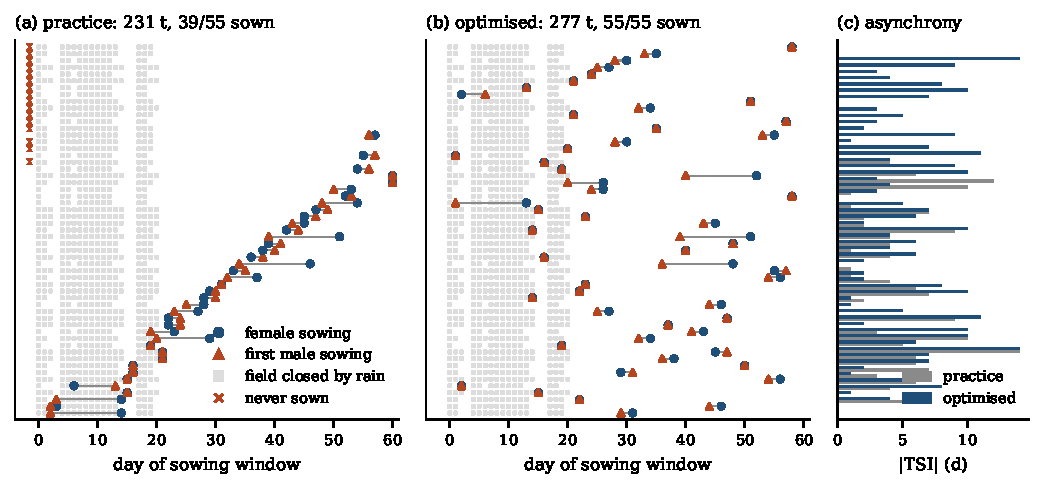
\includegraphics[width=\columnwidth]{../figs/fig12_practice.pdf}
\caption{What the tool changes. One farm ($N = 70$, $K = 2$, $\pi = 1.72$).
(a) Practice holds every field to its recommended offset, fills the window
from the front, exhausts the agronomically admissible early days and
abandons 48 of 70 fields. (b) The exact assignment relaxes the offset on
some fields and places 42. Crosses mark fields never sown.}
\label{fig:practice}
\end{figure}

\subsection{Is an exact solver needed?}

The greedy dispatcher receives the same candidate set and differs only in
assigning fields one at a time, hardest cross first. Against practice as
described it looks useful ($+6.6$\% pooled); against the best hand rule it
is \emph{worse}, $-9.6$\% pooled (95\% CI $-11.0$ to $-8.1$) and worse at
every $N$ from 35 up. Taking the best slot for each hard field in turn
spends the contested early days on synchrony and leaves later fields nowhere
to go. No one-field-at-a-time rule can make the joint trade, and the exact
solve costs seconds (4.7\,s at $N = 70$, 22{,}677 binaries).

\subsection{Robustness: yield response and visit accounting}

Three parts of the scored response are contested rather than measured ---
which published regression, how wide the plateau, how steep the reflection
--- and the visit accounting is an assumption about the crew's scarce
resource. We test both, rebuilding the candidate set under each setting so
objective and scorer agree.

\begin{table}[t]
\caption{Exact assignment with visit merging disallowed}
\label{tab:robust}
\centering
\footnotesize
\setlength{\tabcolsep}{3.4pt}
\begin{tabular}{@{}lrrrr@{}}
\hline
 & \multicolumn{2}{c}{$N = 40$} & \multicolumn{2}{c}{$N = 70$} \\
\cmidrule(lr){2-3}\cmidrule(lr){4-5}
 & allowed & forbidden & allowed & forbidden \\
\hline
gain over best of four orders & $+26.9$ & $+20.3$ & $+37.4$ & $+23.3$ \\
fields sown by the exact plan & 36 & 29 & 42 & 29 \\
merged fraction of chosen plans & 0.58 & 0 & 0.88 & 0 \\
\hline
\end{tabular}
\\[2pt]
\footnotesize\raggedright Gains per cent, mean over three farms. The
baseline is the best of the \emph{four} service orders, without the
offset-relaxing rule of Table~\ref{tab:solution}, so these are not directly
comparable with that table's $+35.2$\% at $N = 70$.
\end{table}

Over the eighteen-cell scenario grid at $N = 70$ (two curves $\times$ three
plateaus $\times$ $\kappa \in \{1.5, 2.0, 2.5\}$, three farms each, all 54
solves optimal with gaps below $0.0005$) the gain over the best of four
service orders runs from $+28.6$\% to $+44.9$\%, mean $+38.7$\%, and is
\emph{positive in every one}; the primary setting is neither the most nor
the least favourable, so the conclusion does not rest on a contested
modelling choice. Merging matters more than is
comfortable to report: forbidding it --- by removing every merged candidate
from the set given to \emph{every} planner, so the comparison stays
like-for-like --- costs the exact plan thirteen of its 42 fields at $N = 70$
and cuts the gain from $+37.4$\% to $+23.3$\%. It does not account for the
result: with every field costing three separate crew-days the
optimiser still beats that baseline by about a fifth at both farm sizes; but
a producer whose crew is limited by rows sown rather than visits to isolated
fields should expect the smaller figure.

\subsection{What in-season replanning is worth}
\label{sec:replan}

Re-solving on the fields not yet sown, at four points through the window and
over the same ensemble candidate set, gives a mean gain of $+0.004$\% across
nine configurations ($N = 30, 45, 70 \times$ three farms; maximum
$+0.026$\%). That is solver tolerance, and it is what theory predicts: the
static solve is already globally optimal over that candidate set, so
re-solving a sub-problem of it with the same information cannot improve on
it.

This bounds the \emph{scheduling-side} value of adaptivity at zero and
locates any remaining value on the \emph{information-side} --- what a
revision is worth when it can use weather observed since sowing began ---
which requires candidate sets conditioned on partially-realised seasons.
Whether the near-null irrigation
results~\cite{kelly2023,becker2026} transfer to an operation where a timing
error costs the whole crop is therefore open.

% =========================================================================
\section{Discussion}
\label{sec:limits}
\label{sec:iot}
% =========================================================================

\emph{Solve the assignment before the season wherever the crew is the
binding constraint.} The deployment test is a single division: compute
$\pi = 3N/TK$. Below about $\pi = 0.5$ exact scheduling adds nothing
measurable over a good hand rule, and a supervisor's calendar is sufficient.
At or above it the exact assignment yields $+20.8$\% over the best hand rule
and $+35.2$\% at the largest farm tested, needs no forecast, no in-season
data collection and no change to agronomy, and runs in seconds on free
software. The steepness of the measured yield response to asynchrony
\eqref{eq:yield} is what makes the placement decision worth solving jointly
rather than field by field.

\emph{Per-field soil-temperature sensing earns its cost only under the same
scarcity.} A simulated probe that resolves the field-specific gap the CERES
imputation leaves unfilled (Section~\ref{sec:formulation}) gains $+0.563$\%
$[+0.392,+0.735]$, positive in all six seeds, once the crew is the binding
constraint ($N=60$, $\sigma=0.7^\circ$C), against an oracle ceiling of
$+2.279$\%; without a binding capacity constraint the gain is $+0.191$\%
$[-0.008,+0.389]$, an interval spanning zero. Instrument accuracy, not the
scheduler, limits what is captured: a noiseless probe recovers the oracle
exactly, a realistic one about a quarter of it. The between-field
heterogeneity a commercial seed-production block would actually show, and
whether a physical sensor would clear this bar in practice, are not
established here.

\emph{Limitations.} This is a simulation study: no seed was produced and no
schedule of ours executed in the field, so the findings say when these
schedules are worth \emph{testing}, not that a gain will be realised on a
given farm. Current practice is described, not observed, from the agronomic
recommendations and the operational assumption they
state~\cite{chassaigne2021}; because that rule is the weakest a supervisor
could follow, every result is also reported against the best of five hand
rules, and that is the figure we claim. The farms are synthetic: weather,
site and crop model are real, but areas, drainage classes, parent pairs and
capacity are sampled, and the parents are public DSSAT cultivars rather than
proprietary inbreds. A producer's calibration would shift the offsets
without changing the structure of the result, which depends on how variable
the parent flowering gap is across seasons and on how hard the crew is
worked, not on the gap's mean; under water or nitrogen stress, not
simulated, asynchrony would be larger and more weather-dependent. The yield
response is from Chitwan, Nepal, applied at a Karnataka site, and is the
only published quantitative seed-yield-versus-TSI response we could find;
its early-TSI branch is a declared reflection, not a fit, with only its
\emph{ordering} constrained by data through $\kappa > 1.43$. Its coefficients
are a published fit we cannot re-estimate: four treatment means are available
to us against three free parameters. Refitting through each three-point
subset preserves the direction of the result --- positive in all 54 cells,
weakest cell $+13.5$\% --- while moving its size: the mean advantage over the
best hand rule is $+28.5$\% and $+39.5$\% under the two subsets that keep a
declining convex response, against $+39.1$\% for the published fit. The
remaining two subsets invert the curvature and flatten the response to no
synchrony penalty, so they test a different model rather than this one. We score mass
rather than saleable seed and model one lever; nitrogen to the late parent
would require replacing the objective, since it changes seed weight and
hence the grading and germination on which hybrid seed is
sold~\cite{marahatta2025,priyanka2017,patil2026}. Crew capacity is counted
in field-visits, so two parent sowings on one field on one day are one visit
--- right if the scarce resource is the supervised unit's presence at an
isolated field, but if it were rows sown, about a third of the advantage
would not be available.

\section{Conclusion and Future Work}
% =========================================================================

We formulated the supervisor's hand decision --- which field a shared sowing
crew starts on which day --- as a stochastic assignment problem, solved it
exactly, and evaluated it on twenty-one observed seasons with flowering
dates from CERES-Maize. The result is conditional, and the condition is the
finding: under slack capacity the best of five hand rules comes within
$0.2$\% of exact optimisation, so a supervisor's calendar suffices there.
Once the crew is over-subscribed the exact assignment
is worth $+20.8$\% more than that rule and $+42.5$\% more than described
practice, reaching $+35.2$\% and $+73.3$\% at the largest farm tested. The
reason is not agronomy --- every rule compared carries the correct
per-hybrid offsets --- but that the recommended offset exhausts the
admissible window and abandons the fields arriving late, where the optimiser
concedes a day or two of synchrony on some to place many more. The gain
holds in all 54 cells of the yield-response grid, falls by about a third to
$+23$\% when visit merging is forbidden, and a greedy dispatcher given the
same information is $9.6$\% \emph{worse} than a good ordering rule: the
trade is joint. Replanning over the same information is worth $+0.004$\%,
which places whatever value adaptivity carries in information the static
plan does not hold.

Two things follow. A field trial --- executing one of these schedules on
real fields and weighing the seed --- is the immediate next step. Pricing
adaptivity needs an experiment that supplies information the static plan
lacks and charges for obtaining it, since observation consumes the very
capacity the schedule competes for.

\emph{Reproducibility.} Simulator, weather record, CERES-Maize table,
runners, result files and the 200-test suite are released under MIT at
\textcolor{ieeelink}{\url{https://github.com/Kishore-Gumu2no/Multi-Field-Hybrid-Maize-Seed-Production}};
three documented commands reproduce every scheduling number, and a fourth
recomputes every headline, interval, table cell and solver diagnostic from
the raw rows, all $28/28$ checks passing.

\begin{thebibliography}{99}
\scriptsize\linespread{0.94}\selectfont
\setlength{\itemsep}{0pt}\setlength{\parskip}{0pt}

\bibitem{marahatta2025}
S.~Marahatta, R.~Basnet, S.~Bastola, and P.~R.~Dulal,
``Optimizing male inbred sowing for hybrid maize seed production in winter and
spring,'' \textit{J. Agric. Food Res.}, vol.~24, art.~102350, 2025.

\bibitem{kelly2023}
T.~D.~Kelly, T.~Foster, and D.~M.~Schultz,
``Assessing the value of adapting irrigation strategies within the season,''
\textit{Agric. Water Manage.}, vol.~275, art.~107986, 2023.

\bibitem{becker2026}
C.~J.~Becker \textit{et al.},
``Optimizing irrigation and fertilization strategies for crop growth under
weather uncertainty,'' \textit{Arch. Comput. Methods Eng.}, 2026.

\bibitem{laurent2025}
A.~Laurent \textit{et al.},
``Predicting inbred parent synchrony at flowering for maize hybrid seed
production by integrating crop growth model with whole genome prediction,''
\textit{Crop Sci.}, 2025.

\bibitem{chassaigne2021}
A.~A.~Chassaigne-Ricciulli \textit{et al.},
``Effective seed yield and flowering synchrony of parents of CIMMYT
three-way-cross tropical maize hybrids,'' \textit{Agriculture}, vol.~11,
no.~2, art.~161, 2021.

\bibitem{fonseca2004}
A.~E.~Fonseca \textit{et al.},
``Simulating potential kernel production in maize hybrid seed fields,''
\textit{Crop Sci.}, vol.~44, pp.~1696--1709, 2004.

\bibitem{khalilzadeh2022}
Z.~Khalilzadeh and L.~Wang,
``Corn planting and harvest scheduling under storage capacity and growing
degree units uncertainty,'' \textit{Sci. Rep.}, vol.~12, no.~1, pp.~1--20, 2022.

\bibitem{rollinghorizon2023}
F.~Montenegro-Dos Santos \textit{et al.},
``A rolling horizon scheme for rescheduling in agricultural harvest,''
\textit{Comput. Electron. Agric.}, 2023.

\bibitem{chassaigne2020}
A.~A.~Chassaigne-Ricciulli \textit{et al.},
``Development of seed production technology of CIMMYT tropical single cross
maize hybrids,'' \textit{Agriculture}, vol.~10, no.~8, art.~318, 2020.

\bibitem{asefa2024}
G.~Asefa \textit{et al.},
``Evaluating released maize hybrid parents for yield producibility and
nicking time in Ethiopia,''
\textit{SVU-Int.\ J.\ Agric.\ Sci.}, vol.~6, no.~3, pp.~1--12, 2024.

\bibitem{priyanka2017}
M.~Priyanka \textit{et al.},
``Influence of synchronization techniques and dates of sowing on nicking in
parental lines of pearl millet hybrid BPMH-3 seed production,''
\textit{Adv.\ Crop Sci.\ Technol.}, vol.~5, no.~4, 2017.

\bibitem{patil2026}
N.~B.~Patil \textit{et al.},
``Optimizing hybrid seed yield in sunflower hybrid KBSH-78 through flowering
synchronization and nitrogen management,'' \textit{J.\ Adv.\ Biol.\
Biotechnol.}, 2026.

\bibitem{varma2018}
R.~L.~Varma \textit{et al.},
``Method optimization for parental line synchronization in hybrid rice seed
production,'' \textit{Int.\ J.\ Curr.\ Microbiol.\ Appl.\ Sci.}, vol.~7,
pp.~1--8, 2018.

\bibitem{sun2023}
J.~G.~Sun \textit{et al.},
``Optimization model and application for agricultural machinery systems based
on timeliness losses of multiple operations,'' \textit{Agriculture},
vol.~13, no.~7, art.~1317, 2023.

\bibitem{bagheri2025}
P.~Bagheri Tookanlou \textit{et al.},
``Predicting readiness of arable land and scheduling of tillage operations,'' \textit{Oper. Res.}, vol.~25, 2025.

\bibitem{lambrechts2007}
O.~Lambrechts, E.~Demeulemeester, and W.~Herroelen,
``Proactive and reactive strategies for resource-constrained project
scheduling,'' \textit{J.\ Scheduling}, vol.~11, pp.~121--136, 2008.

\bibitem{dssat}
J.~W.~Jones \textit{et al.},
``The DSSAT cropping system model,'' \textit{Eur. J. Agron.}, vol.~18, pp.~235--265, 2003.

\bibitem{power}
NASA Langley Research Center, ``POWER Project: daily meteorological data,''
\url{https://power.larc.nasa.gov}, accessed 2025.

\bibitem{cbc}
J.~Forrest \textit{et al.}, ``coin-or/Cbc: COIN-OR branch-and-cut solver,''
Zenodo, 2024.

\bibitem{iscs2013}
Central Seed Certification Board, \textit{Indian Minimum Seed Certification
Standards}, Dept.\ Agric.\ \& Coop., Min.\ Agric., Govt.\ of India, 2013.

\end{thebibliography}

\end{document}
